\documentclass[11pt,letterpaper]{article}

\usepackage{graphicx}
\usepackage{mathpazo}

\usepackage{minted}
\usemintedstyle{arduino}

\usepackage{geometry}
\geometry{margin=1in}

\title{Difference Plot GNUPlot Output and Code}
\author{Alex Striff}
\date{August 26, 2018}

\begin{document}
\maketitle

\begin{figure}[H]
  \centering
  \colorbox{white}{%
    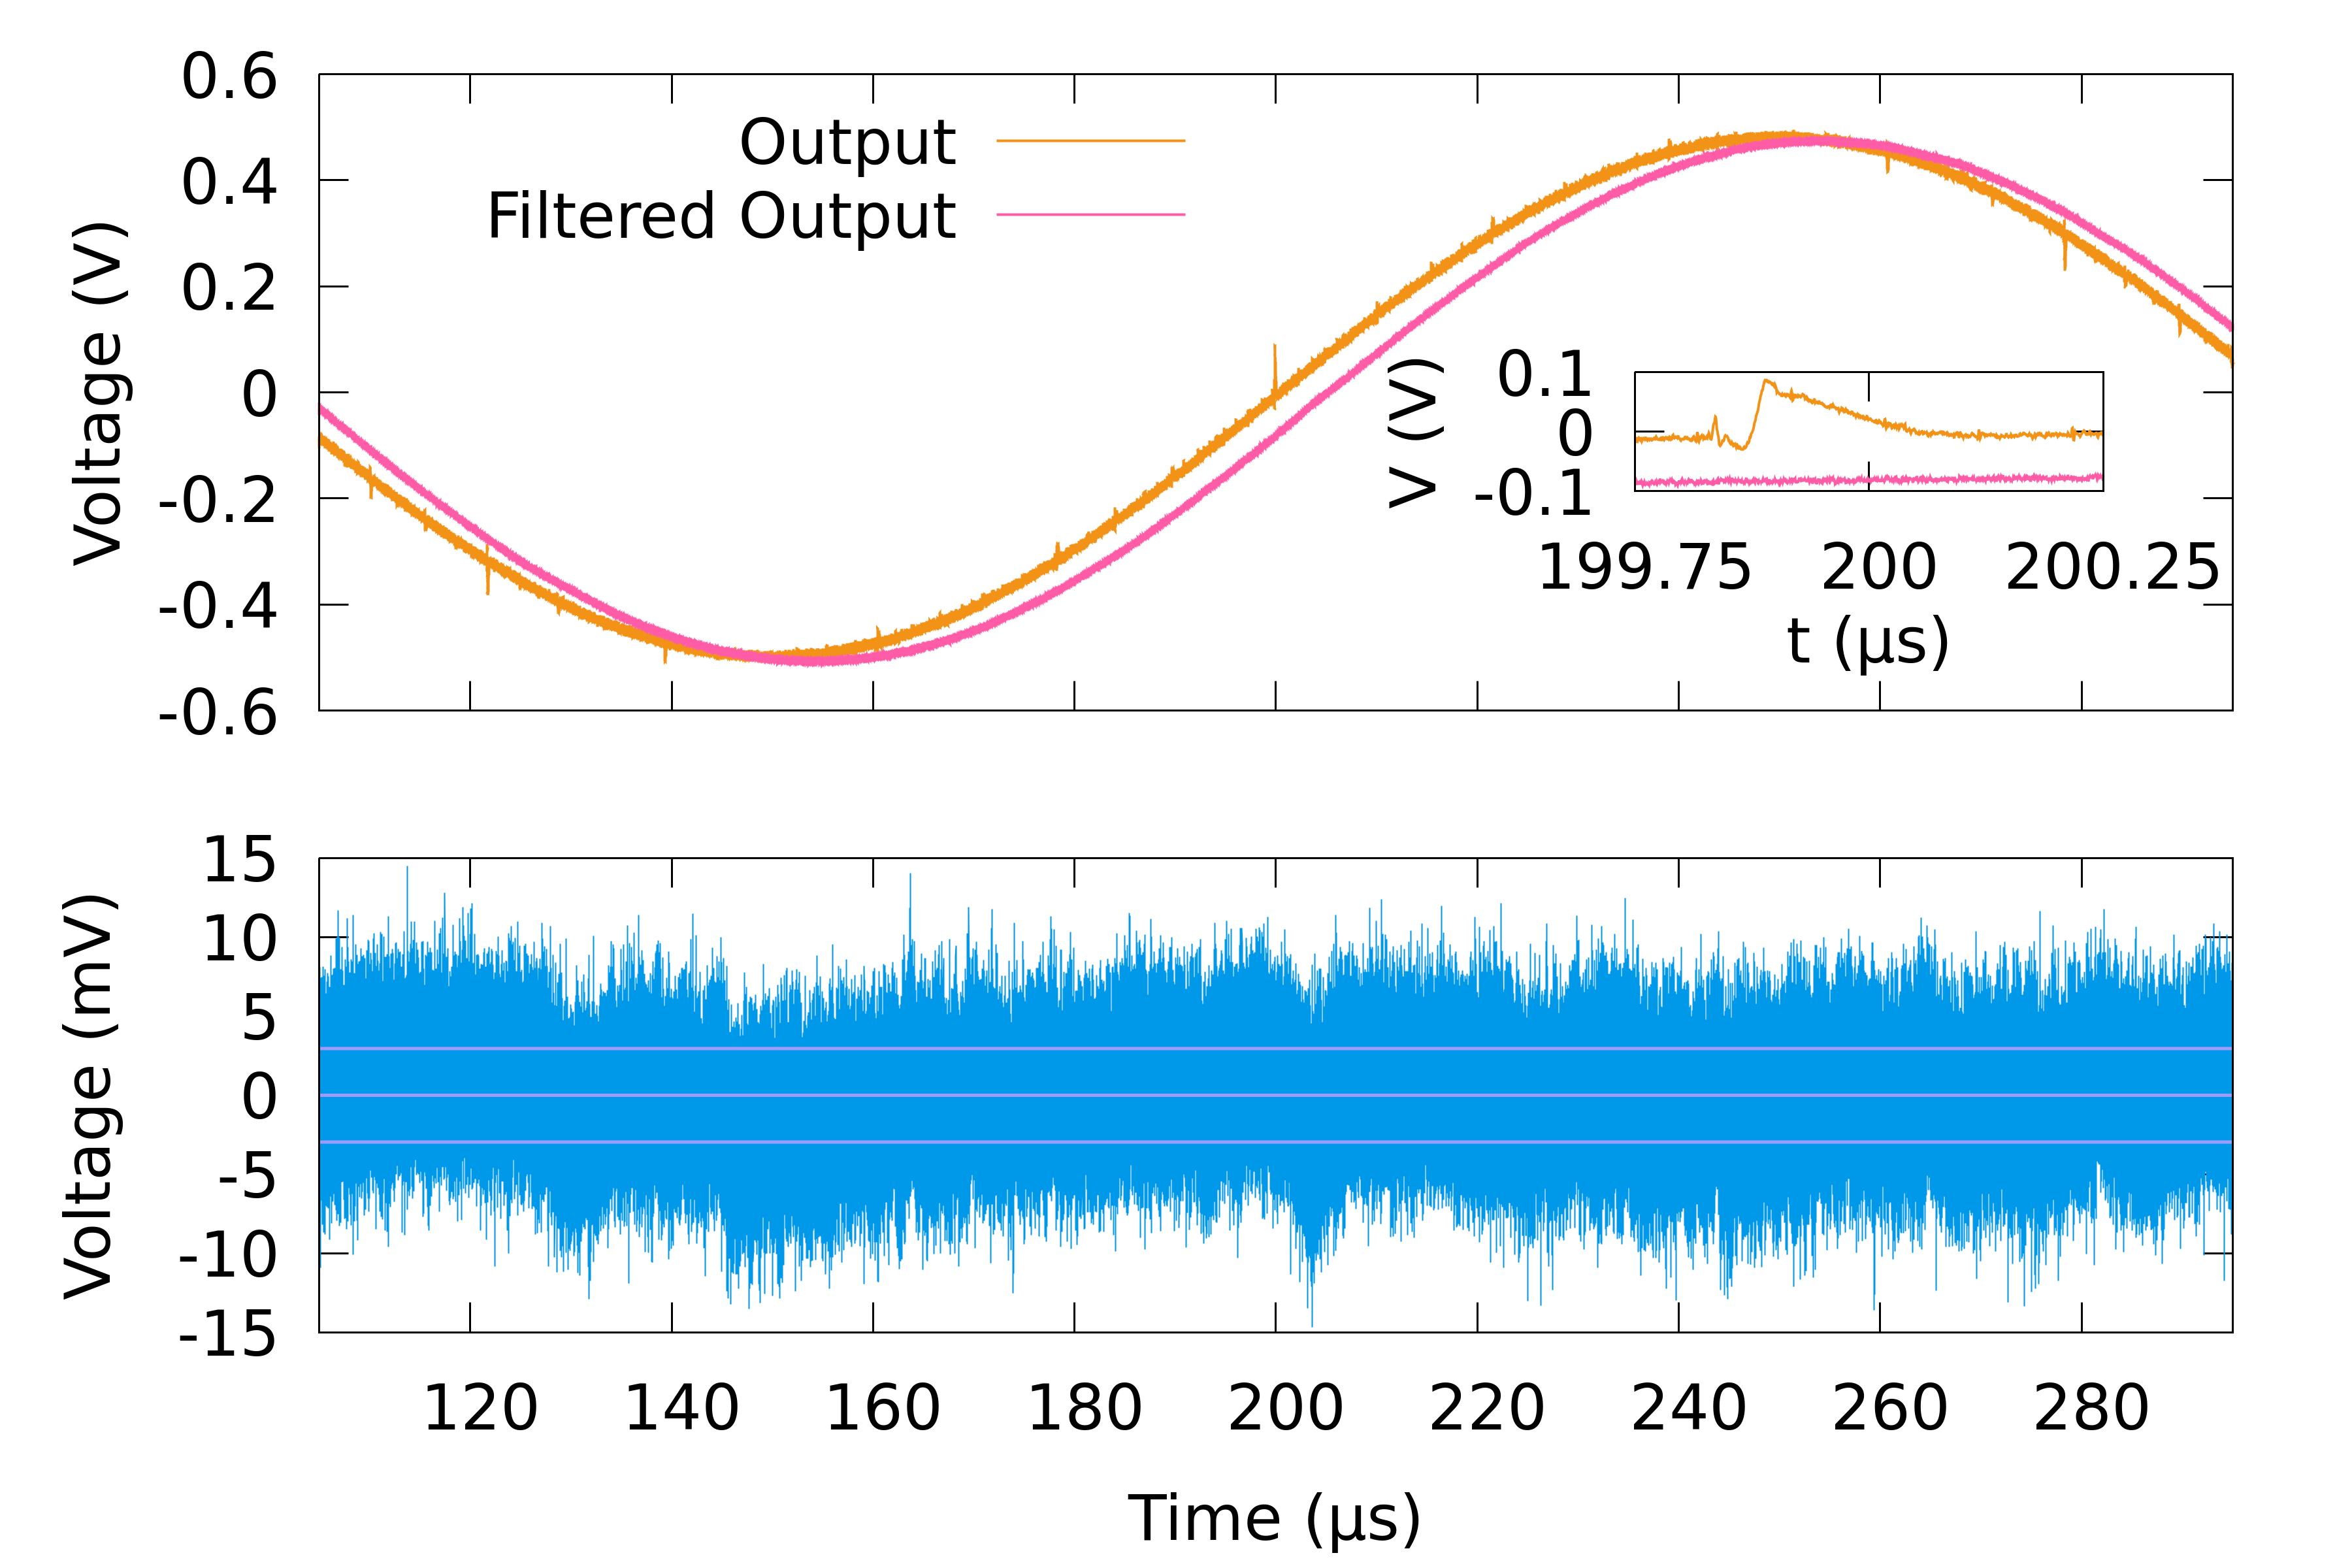
\includegraphics[width=\linewidth]{../diffplot-pc.png}
  }
  \caption{Paper, color version.}
\end{figure}
\begin{figure}[H]
  \centering
  \colorbox{white}{%
    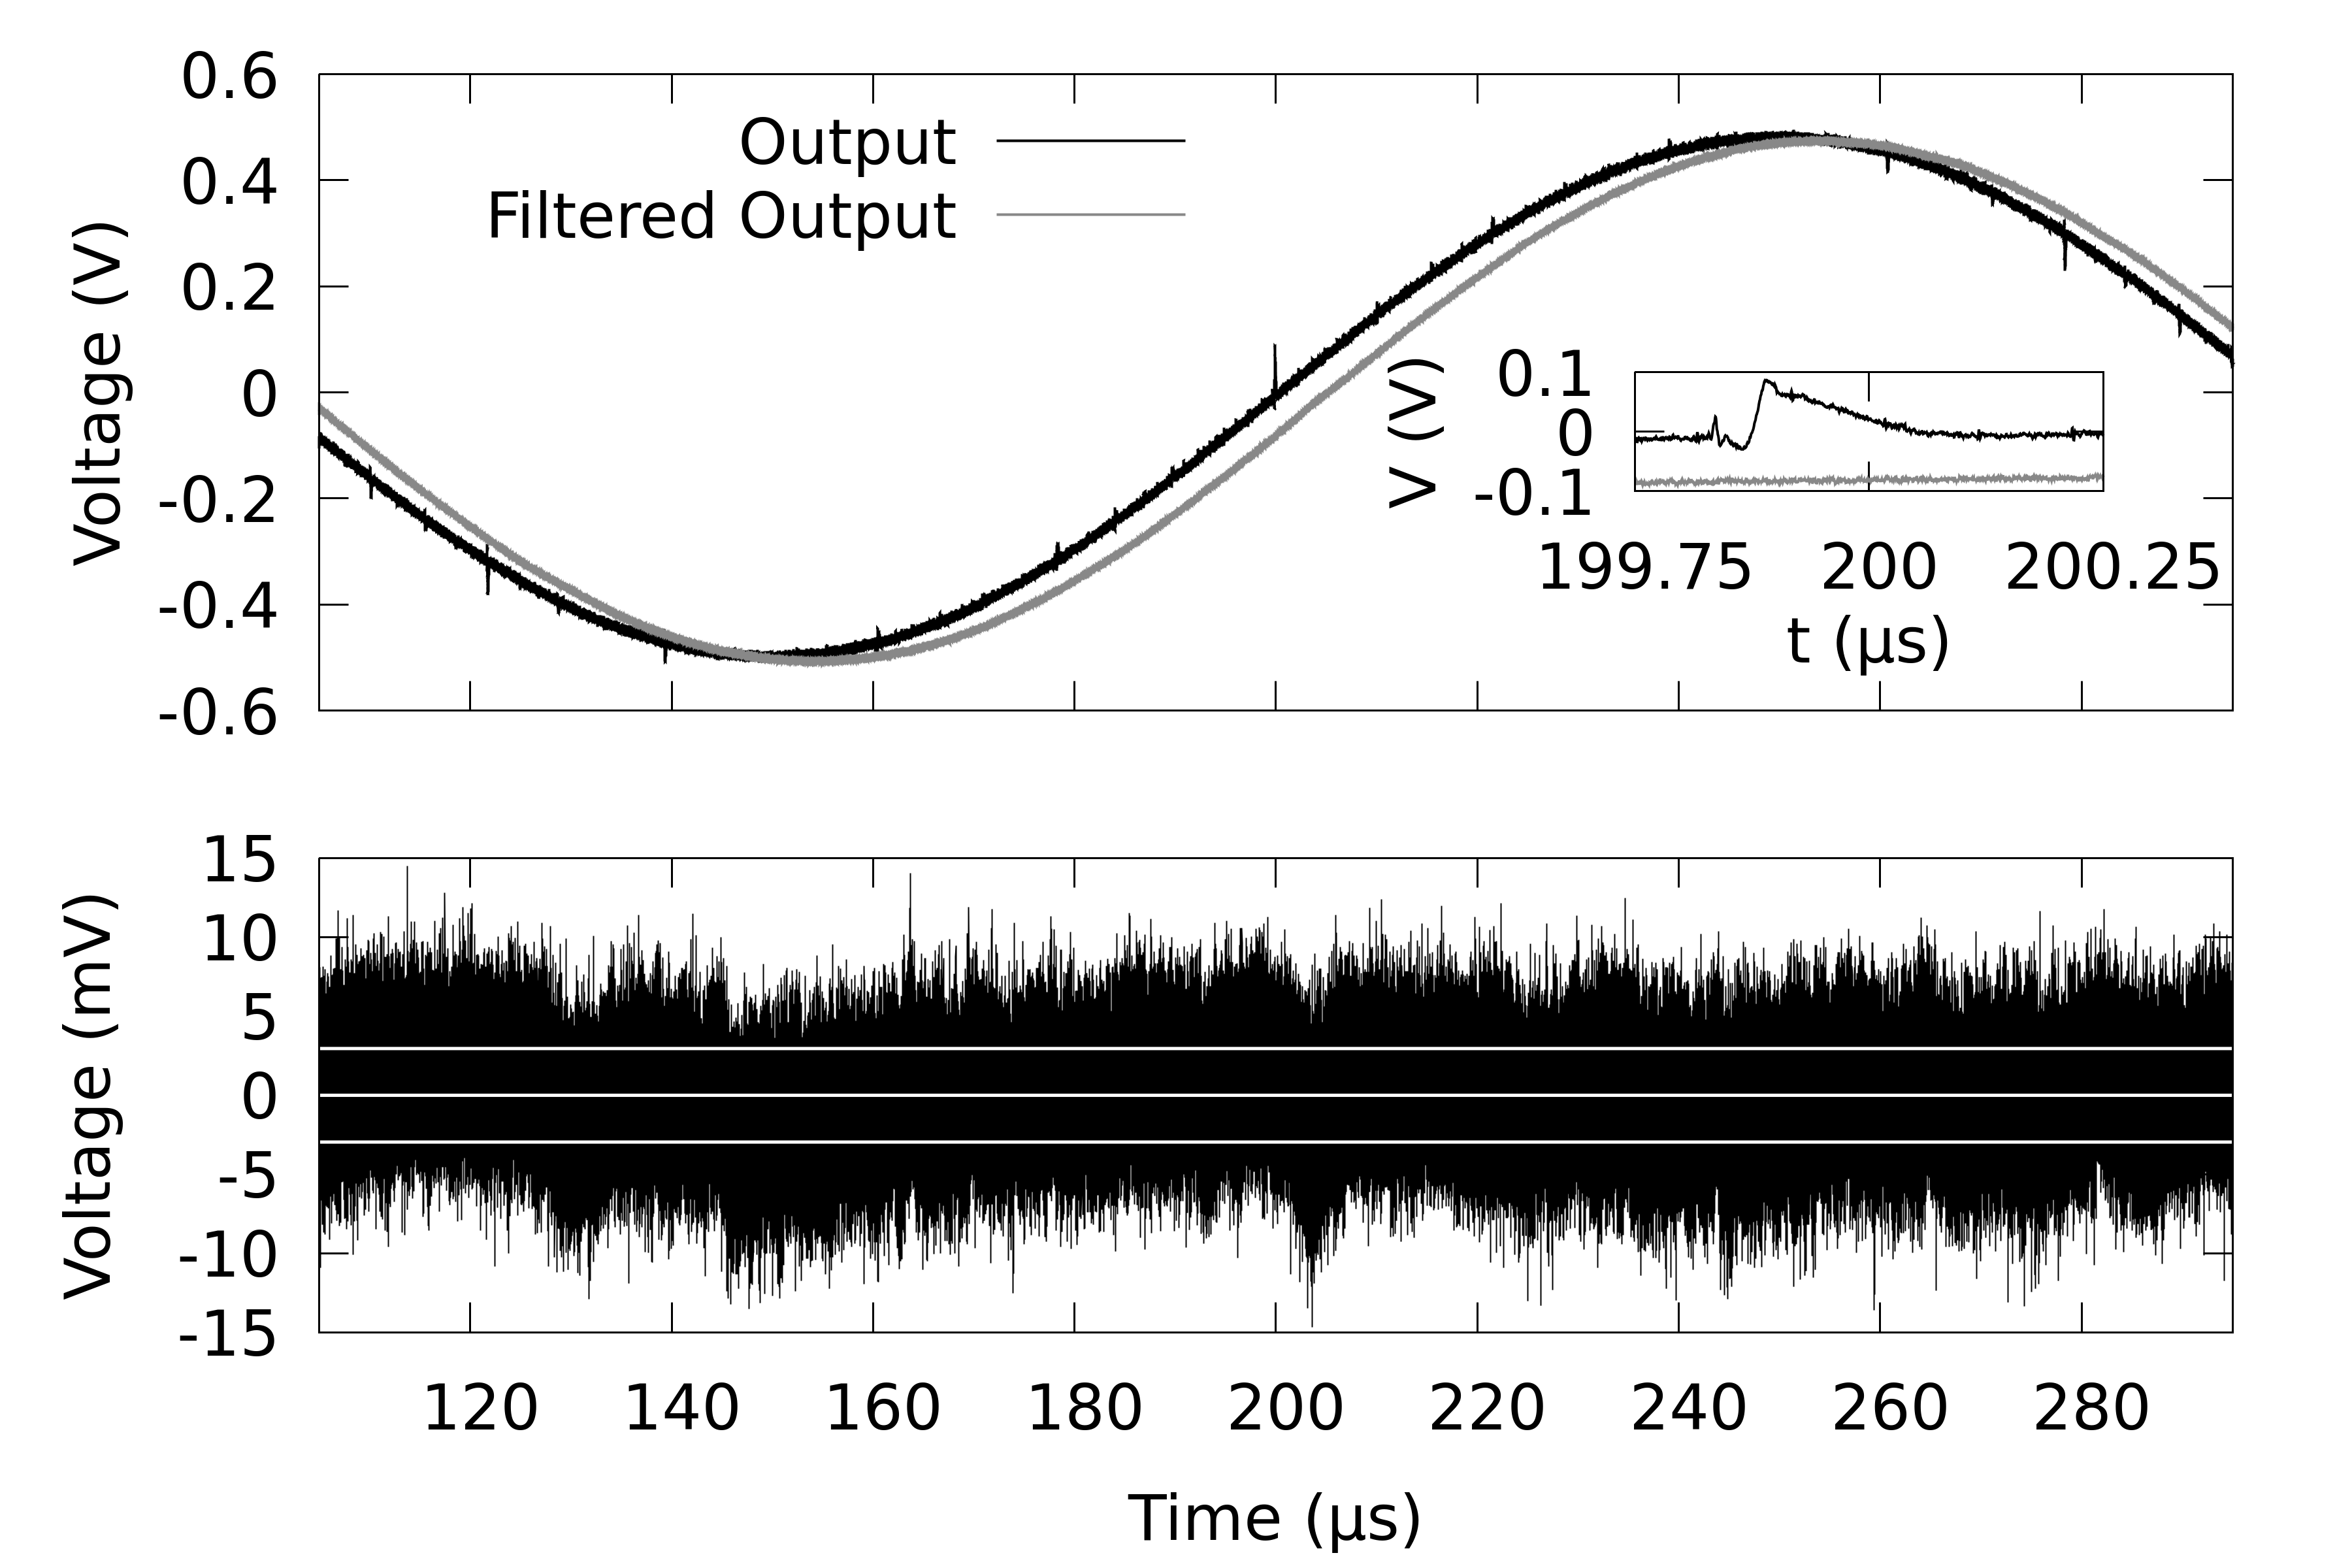
\includegraphics[width=\linewidth]{../diffplot-pg.png}
  }
  \caption{Paper, grayscale version.}
\end{figure}
\begin{figure}[H]
  \centering
  \colorbox{black}{%
    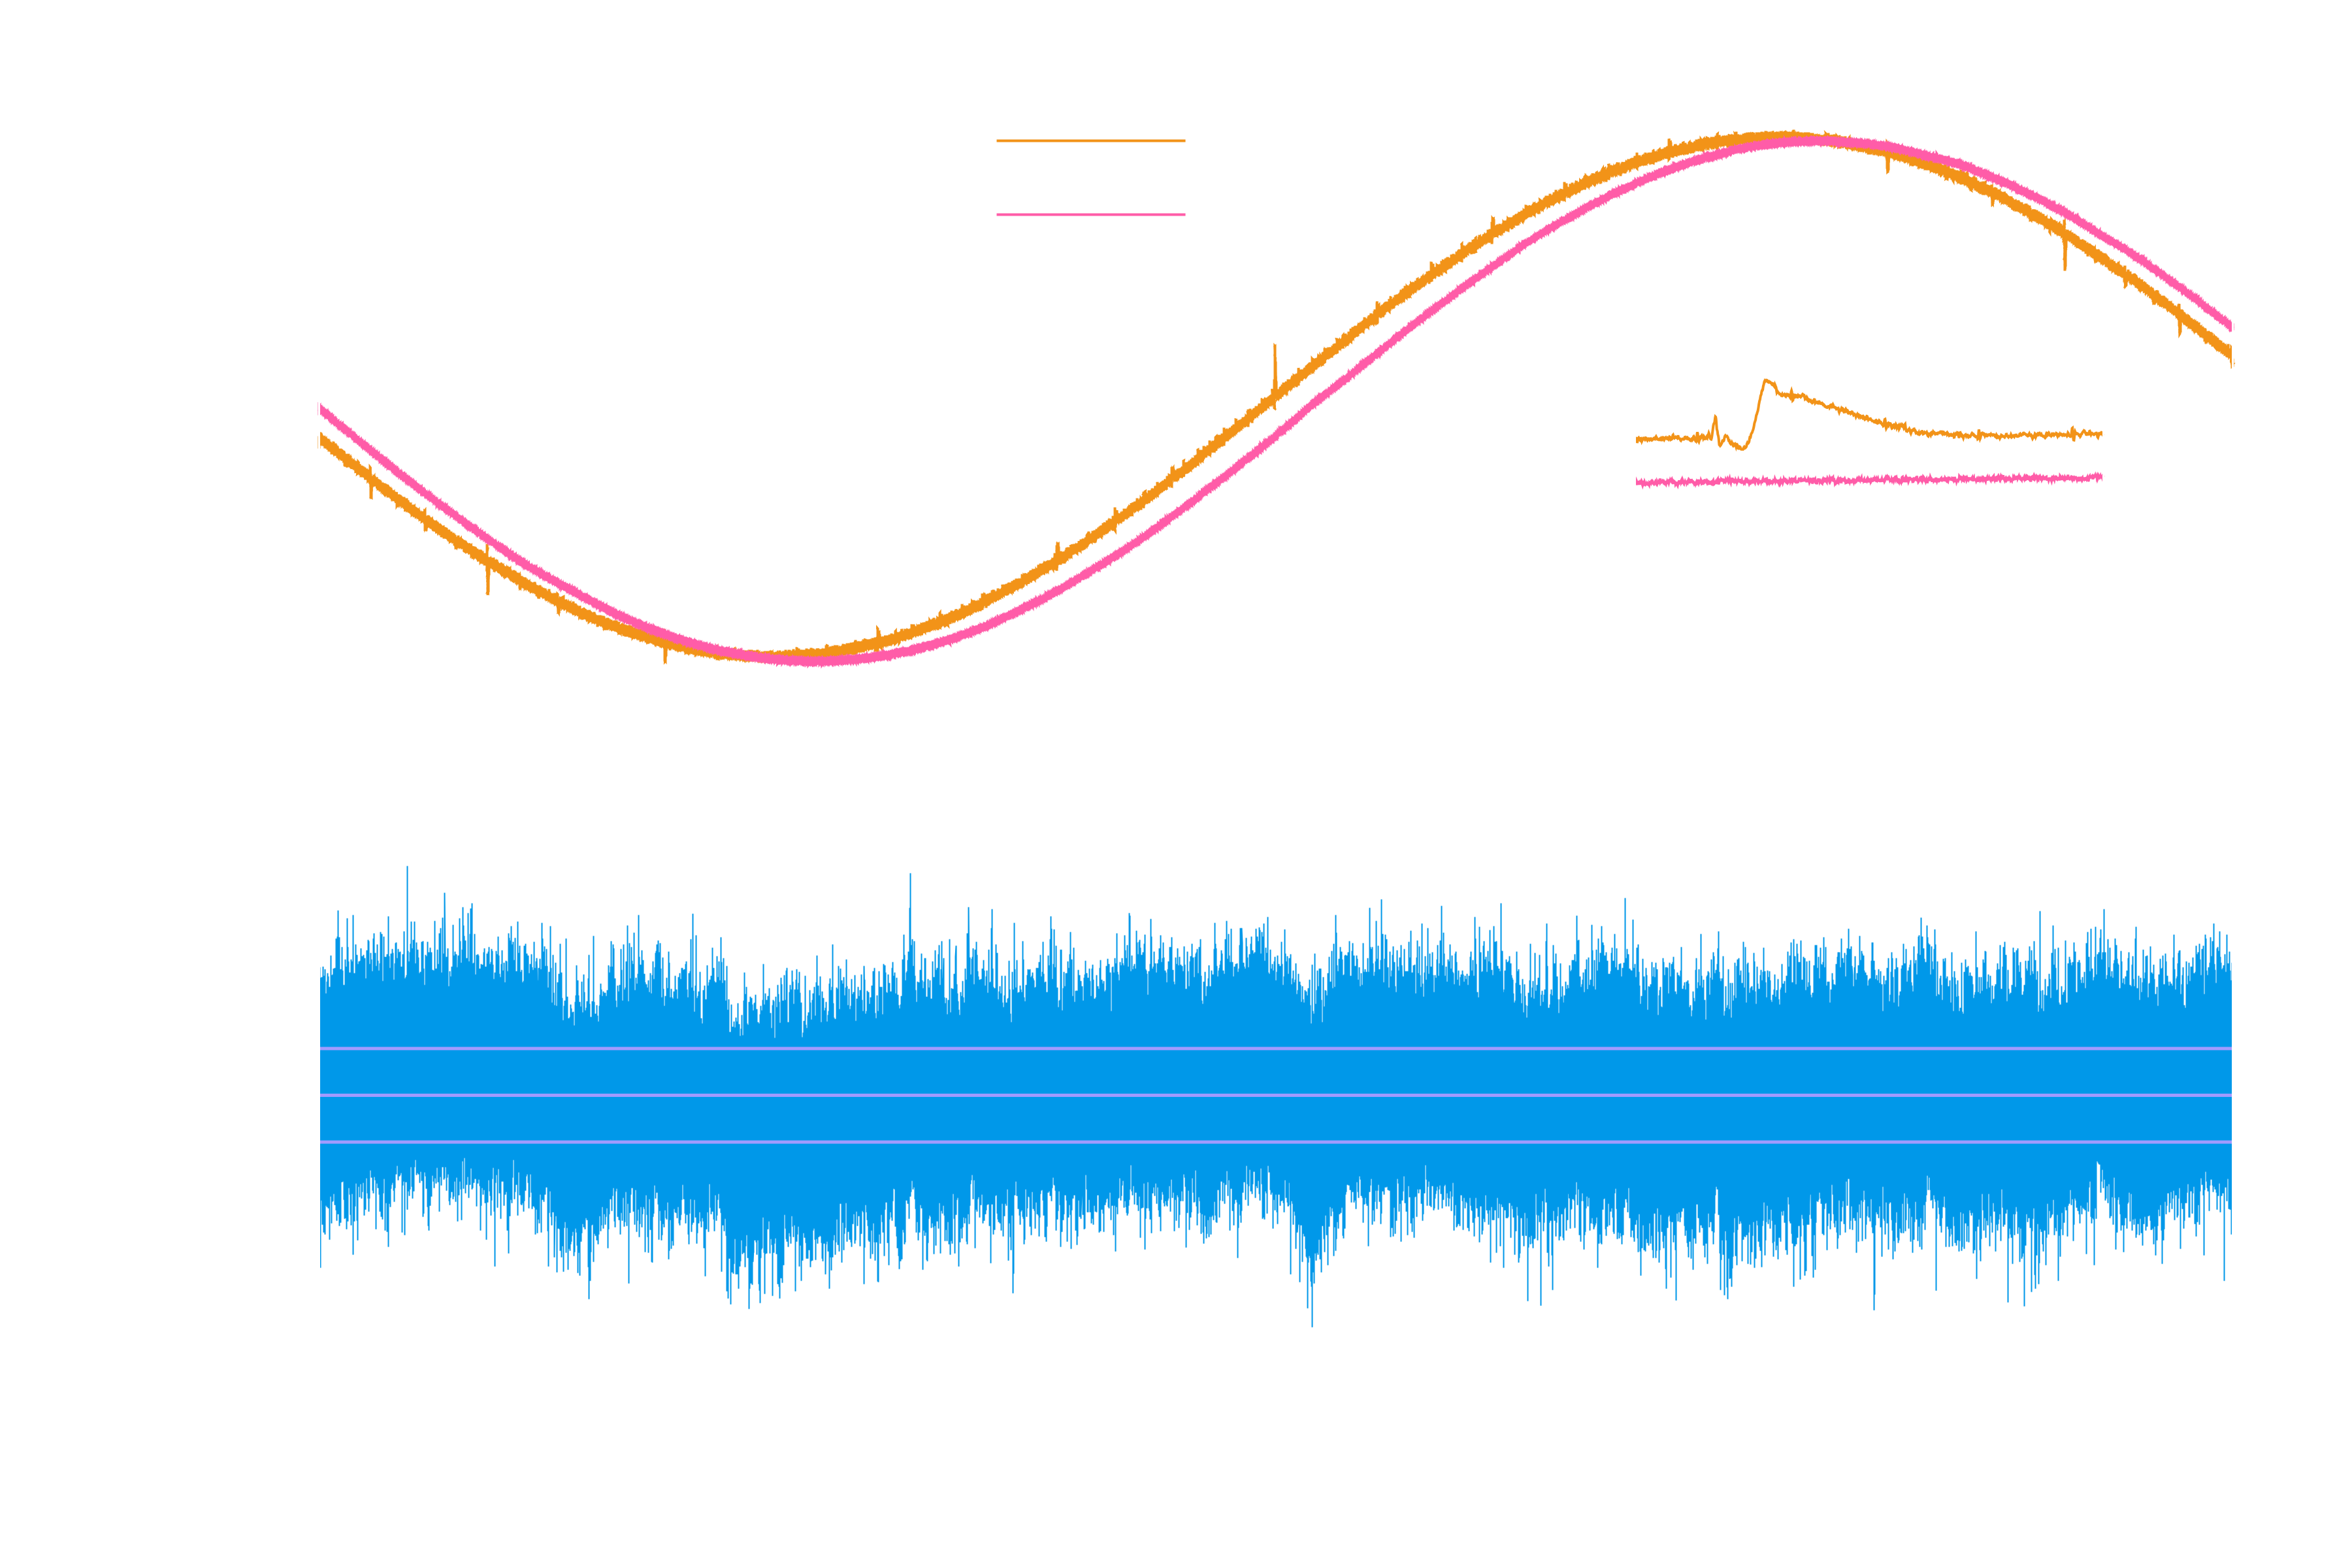
\includegraphics[width=\linewidth]{../diffplot-do.png}
  }
  \caption{Dark Owl version (beamer slides).}
\end{figure}

\begin{minted}{gnuplot}
set terminal pngcairo transparent enhanced font "Droid Sans,72" \
      fontscale 1.0 size 3600, 2400

# Dark Owl
# text     = '#ffffff'
# aout     = '#f29318' # OwlYellow
# abessel4 = '#ff5ca8' # OwlRed
# adiff    = '#0098e9' # OwlBlue
# horiz    = '#a29bff' # (rgb(OwlRed) .+ rgb(OwlBlue)) norm. to max. blue
# set output 'diffplot-do.png'

# Paper Color
text     = '#000000'
aout     = '#f29318' # OwlYellow
abessel4 = '#ff5ca8' # OwlRed
adiff    = '#0098e9' # OwlBlue
horiz    = '#a29bff' # (rgb(OwlRed) .+ rgb(OwlBlue)) norm. to max. blue
set output 'diffplot-pc.png'

# Paper Grayscale
# text     = '#000000'
# aout     = '#000000'
# abessel4 = '#888888'
# adiff    = '#000000'
# horiz    = '#ffffff'
# set output 'diffplot-pg.png'

set border lw 3 lc rgb text
set key tc rgb text
set xlabel tc rgb text
set ylabel tc rgb text

set multiplot
set style increment default

set datafile separator ','
paout  = 'paout.csv'
padiff = 'padiff.csv'

# Difference
set size   1, 0.5
set origin 0, 0
set lmargin 8
set xtics auto
unset key
set xlabel 'Time (μs)'
set ylabel 'Voltage (mV)'
set xrange [105:295] noreverse writeback
# set xrange [199:201] noreverse writeback # Faster to plot for debugging

plot \
       padiff u 1:2 w lines lw 2 lt rgb adiff, \
       padiff u 1:3 w lines lw 5 lt rgb horiz, \
       padiff u 1:($3 + $4) w lines lw 5 lt rgb horiz, \
       padiff u 1:($3 - $4) w lines lw 5 lt rgb horiz

# Waveforms zoom-in
set size   0.25, 0.25
set origin 0.695, 0.56
set lmargin 0
set xtics auto 0.25
set ytics auto 0.1
unset key
set xlabel 't (μs)' offset 0,0.5
set ylabel 'V (V)' offset 1.25,0
set xrange [199.75:200.25] noreverse writeback

plot \
       paout u 3:($4 * 1e-3) w lines lw 4 lt rgb aout t '', \
       paout u 5:($6 * 1e-3) w lines lw 4 lt rgb abessel4 t ''

# Waveforms
set size   1, 0.5
set origin 0, 0.5
set lmargin 8
set xtics auto format ''
set ytics auto
unset xlabel
set key left top autotitle columnhead
set ylabel 'Voltage (V)'
set xrange [105:295] noreverse writeback
# set xrange [199:201] noreverse writeback # Faster to plot for debugging

plot \
       paout u 3:($4 * 1e-3) w lines lw 4 lt rgb aout t 'Output', \
       paout u 5:($6 * 1e-3) w lines lw 4 lt rgb abessel4 t 'Filtered Output'

unset multiplot

\end{minted}

\end{document}


